\chapter{Probabilistic logic reasoning}

\begin{description}
    \item[Probabilistic logic programming] \marginnote{Probabilistic logic programming}
        Adds probability distributions over logic programs allowing to define different worlds.
        Joint distributions can also be defined over worlds and allow to answer to queries.
\end{description}



\section{Logic programs with annotated disjunctions (LPAD)}
\marginnote{LPAD}

\subsection{Syntax}

\begin{description}
    \item[\texttt{null}] 
        Atom that can only appear in the head of a clause and 
        cancels the clause (i.e. equivalent of not having the clause).
\end{description}

The head of each clause is defined as a disjunction of atoms, each with a probability.
More specifically, each clause has a probability distribution over its head.

\begin{example}
    \phantom{}
    \begin{lstlisting}
    sneezing(X):0.7 ; null:0.3 :- flu(X).
    sneezing(X):0.8 ; null:0.2 :- hay_fever(X).
    \end{lstlisting}
\end{example}


\subsection{Distribution semantics}

\begin{description}
    \item[Worlds] \marginnote{World}
        Given a clause $C$ and a substitution $\theta$ such that $C\theta$ is ground,
        the following operations are defined for LPAD:
        \begin{descriptionlist}
            \item[Atomic choice] \marginnote{Atomic choice}
                An atomic choice $(C, \theta, i)$ is the selection of the $i$-th atom in the head of $C$ for grounding.

            \item[Composite choice] \marginnote{Composite choice}
                A composite choice $\kappa$ is a set of atomic choices.
                The probability of a composite choice is the following:
                \[ \prob{\kappa} = \prod_{(C, \theta, i) \in \kappa} \prob{C, i} \]
                where $\prob{C, i}$ is the probability of choosing the $i$-th atom in the head of $C$.

            \item[Selection] \marginnote{Selection}
                A selection $\sigma$ is a composite choice where an atom from the head of each clause for each grounding has been chosen.
                In other words, a selection can be defined only when the program is ground.

                A selection $\sigma$ identifies a world $w_\sigma$ and has probability:
                \[ \prob{w_\sigma} = \prob{\sigma} = \prod_{(C, \theta, i) \in \sigma} \prob{C, i} \]
        \end{descriptionlist}

        \begin{example}
            Given the program:
            \begin{lstlisting}
    sneezing(X):0.7 ; null:0.3 :- flu(X).
    sneezing(X):0.8 ; null:0.2 :- hay_fever(X).
            \end{lstlisting}

            The possible worlds are:
            \begin{center}
                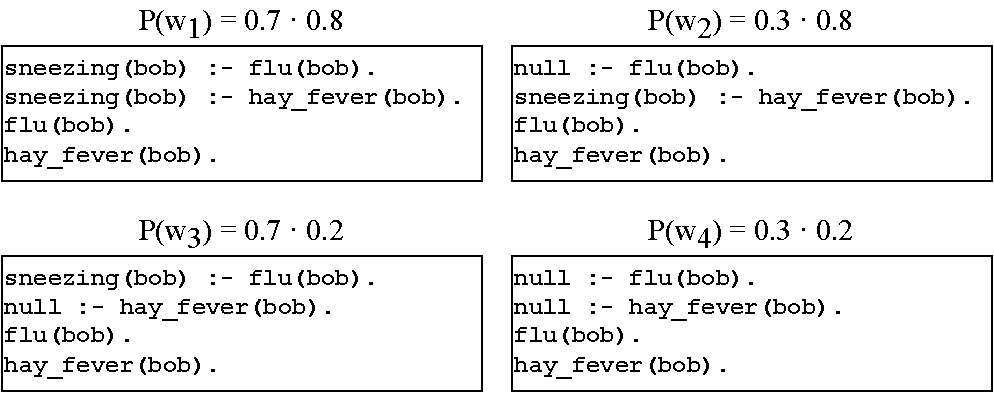
\includegraphics[width=0.7\textwidth]{img/_probabilistic_logic_example.pdf}
            \end{center}
        \end{example}

    \item[Queries] \marginnote{Queries}
        Given a ground query $Q$ and a world $w$, the probability of $Q$ being true in $w$ is trivially:
        \[ 
            \prob{Q \mid w} =
            \begin{cases}
                1 & \text{ if $Q$ is true in $w$}\\
                0 & \text{ otherwise}
            \end{cases} 
        \]

        The overall probability of $Q$ is:
        \[ \prob{Q} = \sum_w \prob{Q, w} = \sum_w \prob{Q \mid w}\prob{w} = \sum_{w \models Q} \prob{w} \]

        \begin{example}
            Given the program:
            \begin{lstlisting}
    sneezing(X):0.7 ; null:0.3 :- flu(X).
    sneezing(X):0.8 ; null:0.2 :- hay_fever(X).
            \end{lstlisting}

            The probability of \texttt{sneezing(bob)} is:
            \[ \prob{\texttt{sneezing(bob)}} = \prob{w_1} + \prob{w_2} + \prob{w_3} \]
        \end{example}
\end{description}